\chapter{Dynamic Tree-Structure Organizations}
\section{B-trees}
\begin{tcolorbox}
A \textit{B-tree} of order \(m\) \((m \geq 3)\) is an \textit{m}-way search tree that is either empty or of height \(h \geq 1\) and it satisfy the following proprieties:
\begin{enumerate}
    \item Each node contains at most \(m - 1\) keys
    \item Each node, except the root, contains at least \( \lceil m/2 \rceil -1\) keys
    \item A node is either a leaf node or has \(j + 1\) children, where j is the number of keys of the node
    \item All leaves appear on same level
    \item Each node has the following structure:
    \[[p_0, k_1*,p_1, k_2*,p_2,...,k_j*,p_j]\]
    where:
    \begin{itemize}
        \item The keys are sorted: \(k_1 < ... < k_j\)
        \item \(p_i\) is a pointer to another node of the tree structure, and is undefined in the leaves
    \end{itemize}
\end{enumerate}
\end{tcolorbox}

\begin{figure}[!h]
    \centering
    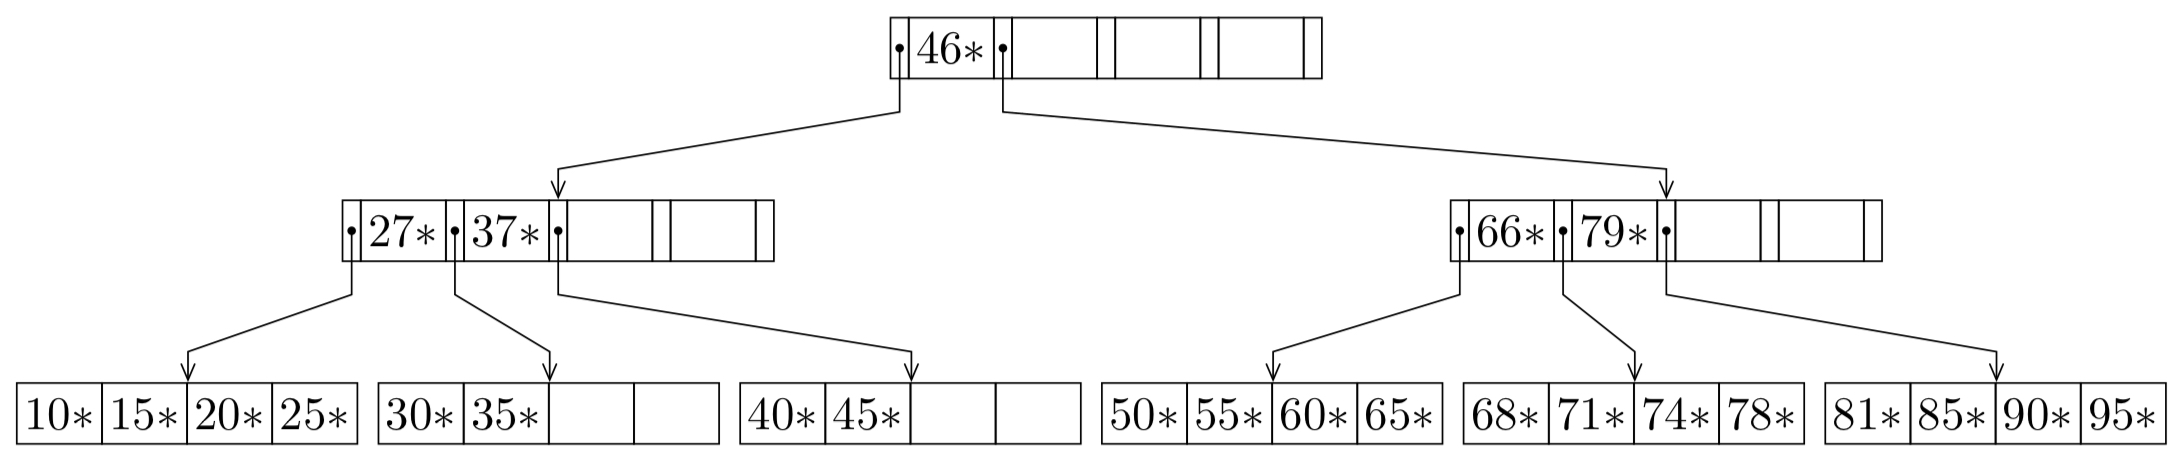
\includegraphics[width=0.99\linewidth]{images/DBMS_Internals/DynamicTreeStructureOrganizations/btree.jpeg}
    \caption{B-tree example}
\end{figure}



\subsection{Operations}

\subsubsection{Search}
The search start at the root node and if the key is not in the root and \(h > 1\) the search continue deeply in the tree like so:
\begin{enumerate}
    \item If \(k_i < k < k_{i+1} \quad 1 \leq i \leq m\) then the search continues in the subtree \(p_i\)
    \item If \(k_m < k\), then the search continues in the subtree \(p_m\)
    \item If \(k < k_1\) the search continues in the subtree \(p_0\)
\end{enumerate}

\subsubsection{Insertion}
\begin{itemize}
    \item First, a search is made for the leaf node which should contain the key \(k\).
    \item An unsuccessful search determines the leaf node \(Q_1\) where \(k\) should be inserted
    \begin{itemize}
        \item If the node \(Q_1\) contains less than \(m - 1\) keys, then \(k\) is inserted and the operation terminates
        \item  Otherwise, if \(Q_1\) is \textbf{full}, it will be split into two nodes, with the \textit{first half} of the \(m\) keys that remain in the old node \(Q_1\), the \textit{second half} of the keys that go into a new adjacent node \(Q_2\), and the median key, together with the pointer to \(Q_2\), that is inserted into the father node \(Q\) of \(Q1\)
    \end{itemize}
\begin{figure}[!h]
    \centering
    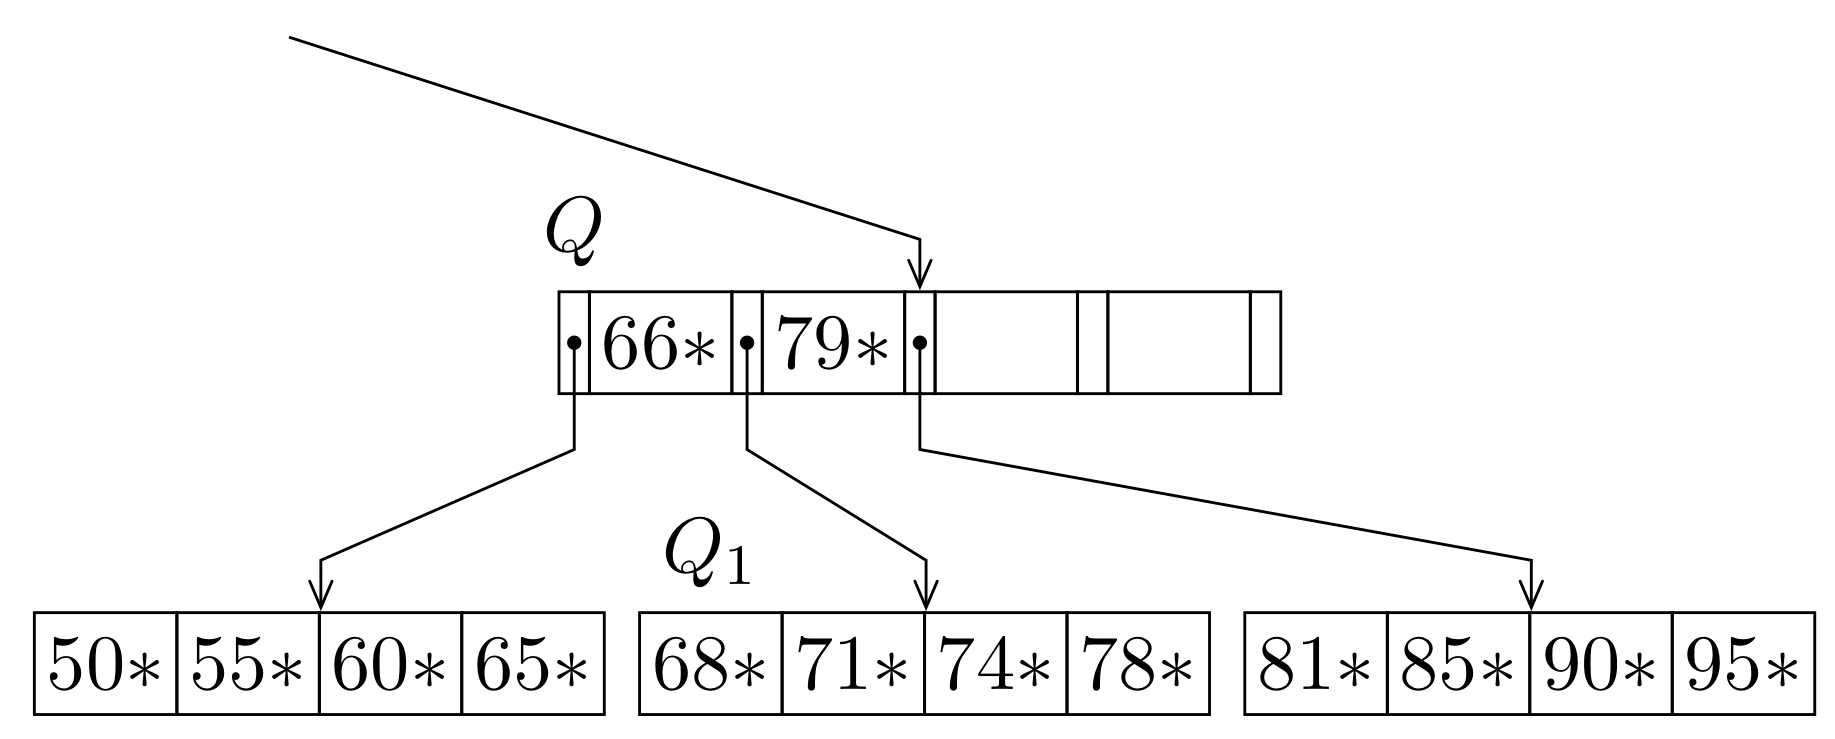
\includegraphics[width=0.5\linewidth]{images/DBMS_Internals/DynamicTreeStructureOrganizations/btree_insertion1.jpeg}
    \caption{Insertion key 70 - Step 1}
\end{figure}

\begin{figure}[!h]
    \centering
    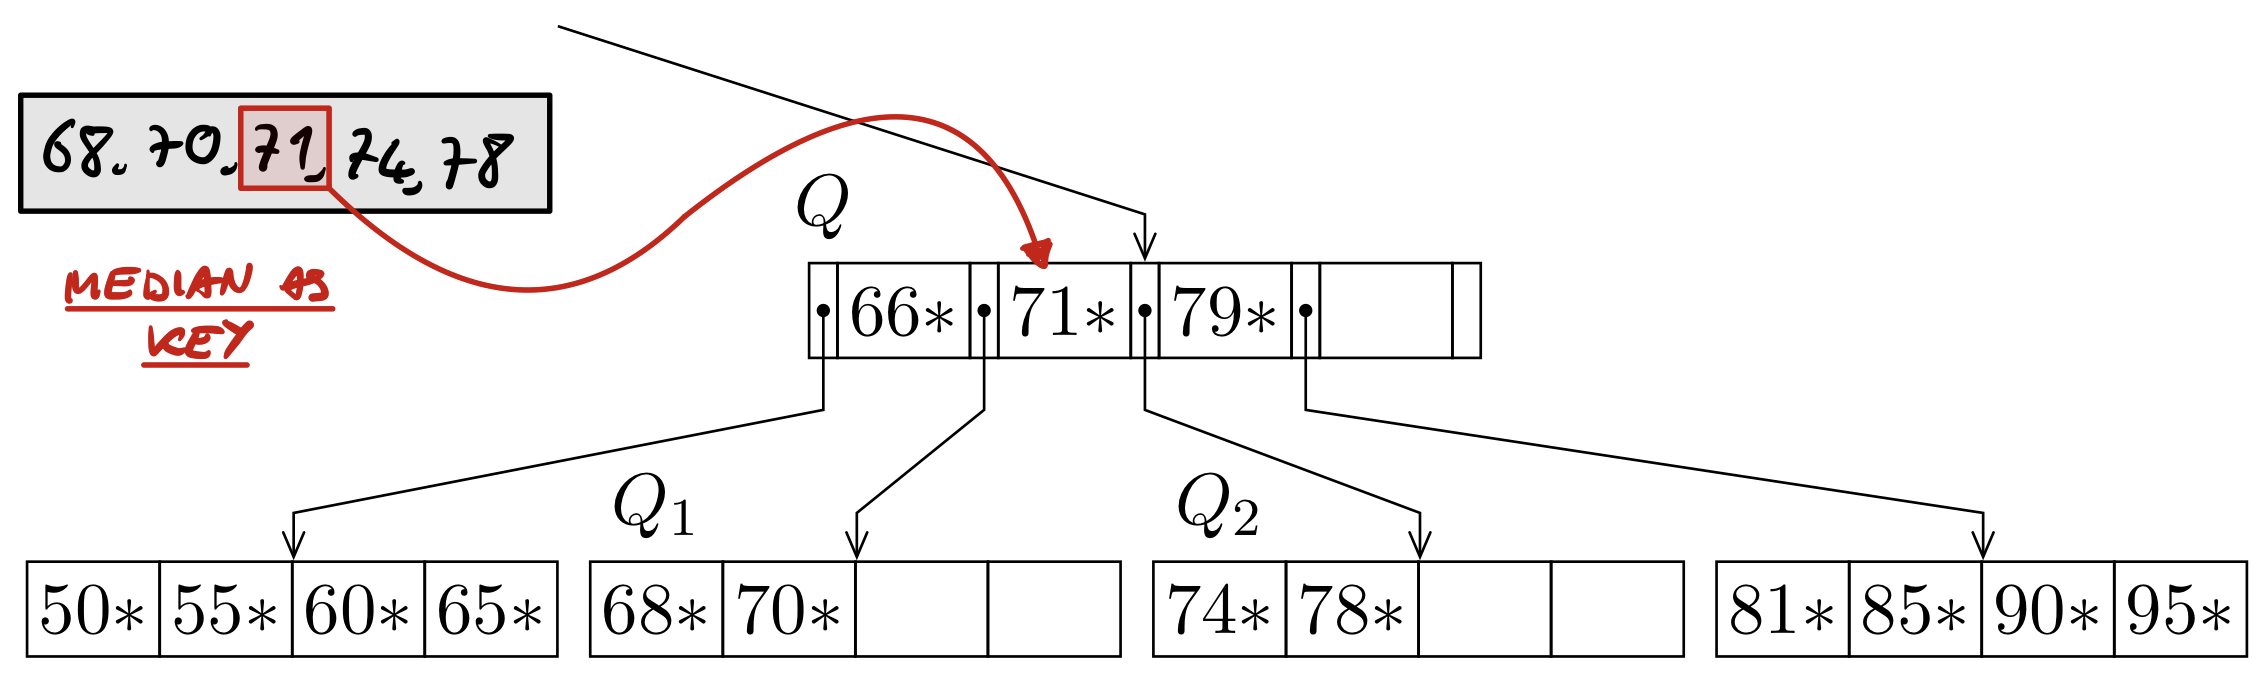
\includegraphics[width=0.5\linewidth]{images/DBMS_Internals/DynamicTreeStructureOrganizations/btree_insertion2.jpeg}
    \caption{Insertion key 70 - Step 2}
\end{figure}

    
\end{itemize}

%%IMAGE

\subsubsection{Deletion}
The deletion is always effected on the leaf nodes. Furthermore, after a deletion if the leaf node \(p\) has less than \(\lceil m/2 \rceil - 1\) keys, it has to be regrouped with an adjacent brother node using one of the following techniques:
\begin{itemize}
    \item \textbf{Merging:} the node \(p\) is \textit{merged} with one of its adjacent brother nodes which contains \(\lceil m/2 \rceil - 1\) elements 
    \item \textbf{Rotation:} when the merging of the node \(p\) with one of its adjacent brothers is not possible, then the \textit{rotation} technique is applied
    \begin{figure}[!h]
    \centering
    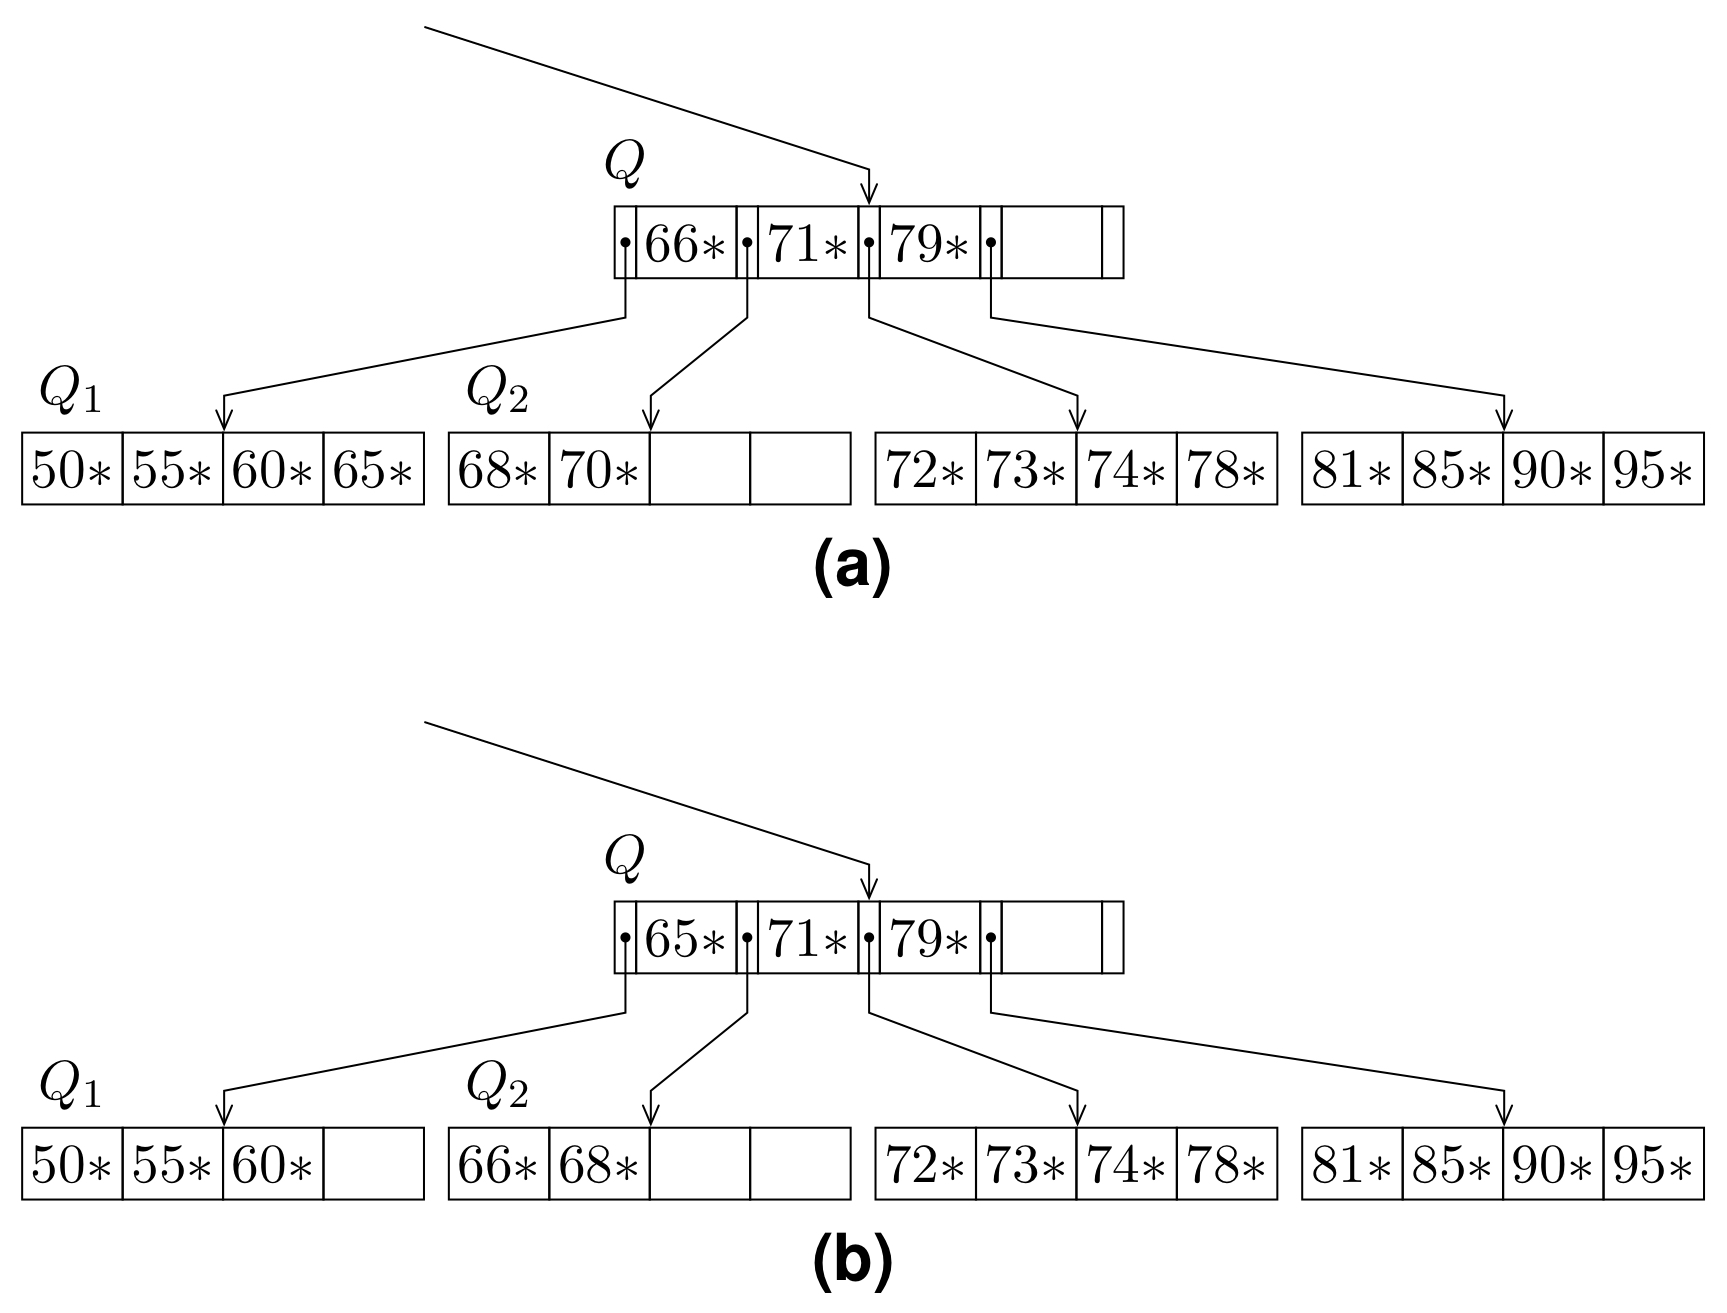
\includegraphics[width=0.6\linewidth]{images/DBMS_Internals/DynamicTreeStructureOrganizations/rotation_example.jpeg}
    \caption{A rotation example}
\end{figure}
\end{itemize}


\section{Performance Evaluation}
Let us evaluate the costs of the operations expressed in terms of the number of nodes to read and write.

\subsection{Search}
The height determines the cost of simple key search since \(1 \leq C \leq h\), and this relation holds:
\[log_m(N +1) \leq h \leq 1 + log_{\lceil m / 2 \rceil} \Bigg(\frac{N + 1}{2} \Bigg)\]

\subsection{Range Search}
B–trees are very good for equality searches, but not to retrieve data sequentially or for range searches, because they require multiple tree traversals.

\subsection{Insertion}
An insertion is made in a leaf node. If the node is not full, the new key is inserted keeping the node’s keys sorted. The cost is h reads and 1 write

\subsection{Deletion}
The cost of the operation is estimated by considering three cases;
\begin{enumerate}
    \item If the key is \textbf{in a leaf} and the \textbf{merging and rotation is not required}, the cost is \(h\) and \(1\) write
    \item If the key is \textbf{in a node} and the \textbf{merging and rotation is not required}, the cost is \(h\) and \(2\) write
    \item The worst case is when for all the nodes of the path from the root to the node, except for the first two, the \textbf{merging} operation is required, and for the child of the root a \textbf{rotation} operation is required, The cost is \(2h - 1\) reads and \(h + 1\) writes
\end{enumerate}


\section{\(B^{+}\)-trees}
A \(B^+\)–tree is a well known B–tree variant to enhance search performance especially for range queries. In a \(B^+\)–tree all the records, denoted as \(k*\), are stored sorted in the leaf nodes, organized int a doubly linked list.

\begin{figure}[!h]
    \centering
    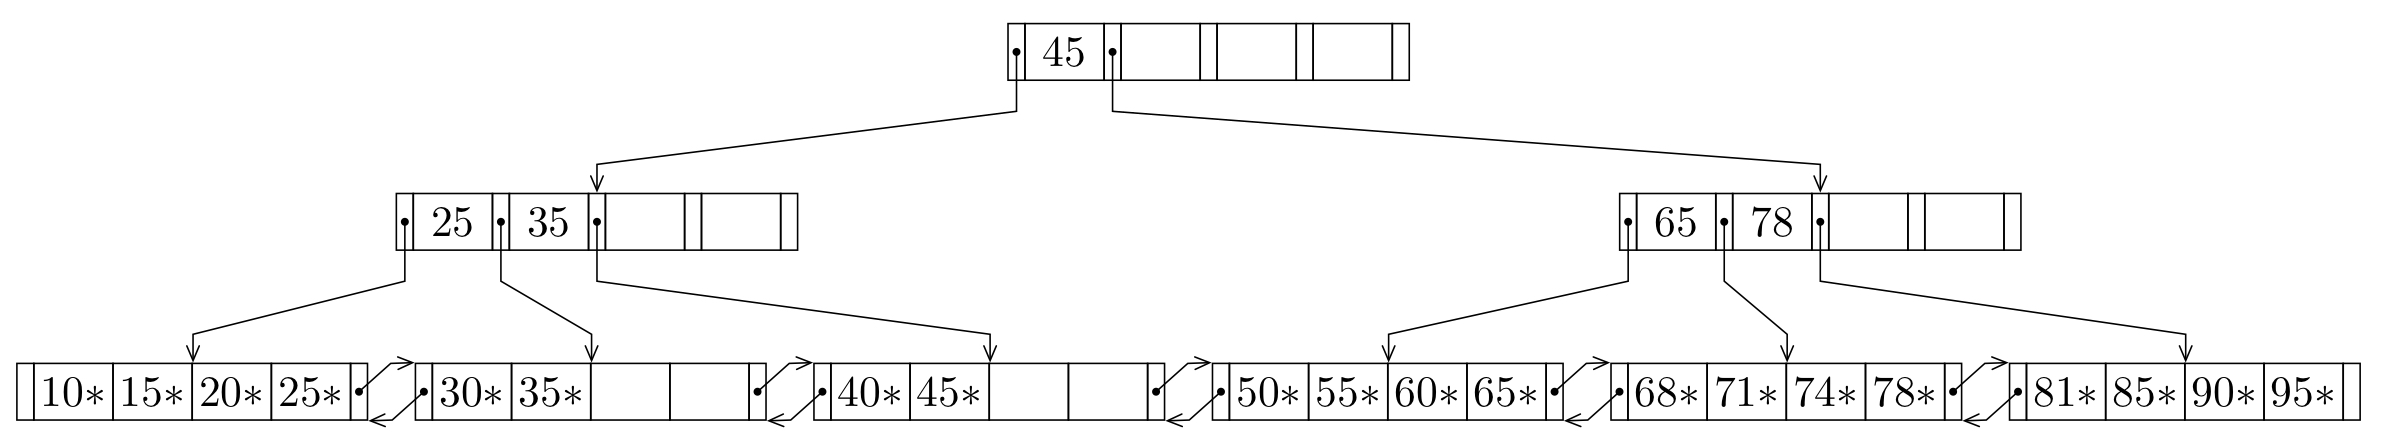
\includegraphics[width=0.99\linewidth]{images/DBMS_Internals/DynamicTreeStructureOrganizations/b+tree.jpeg}
    \caption{B+tree Example}
\end{figure}

\(B^+\)–tree are different from the previous B-tree for the following reasons:
\begin{enumerate}
    \item A key search requires always the same number of accesses equal to the \(B^+\)–tree height
    \item Key search is faster, because the records are stored in the leaf nodes, and only the keys are stored in the non-leaf nodes of the tree
    \item When a leaf node \(F\) is split into \(F_1\) and \(F_2\), a copy of the highest key in \(F_1\) is inserted in the father node of \(F\), while when an internal node \(I\) is split the median key in \(I\) is moved in the father node, as in a B–tree.
    \item When a record with the key \(k_i\) is deleted, the \(k_i*\) is deleted in the leaf \(F\), and if \(k_i\) is used in a father node because it was the highest key in \(F\), it is not necessary to replace it with the new highest key in \(F\)
\end{enumerate}


\section{Index Organization}

\begin{figure}[!h]
    \centering
    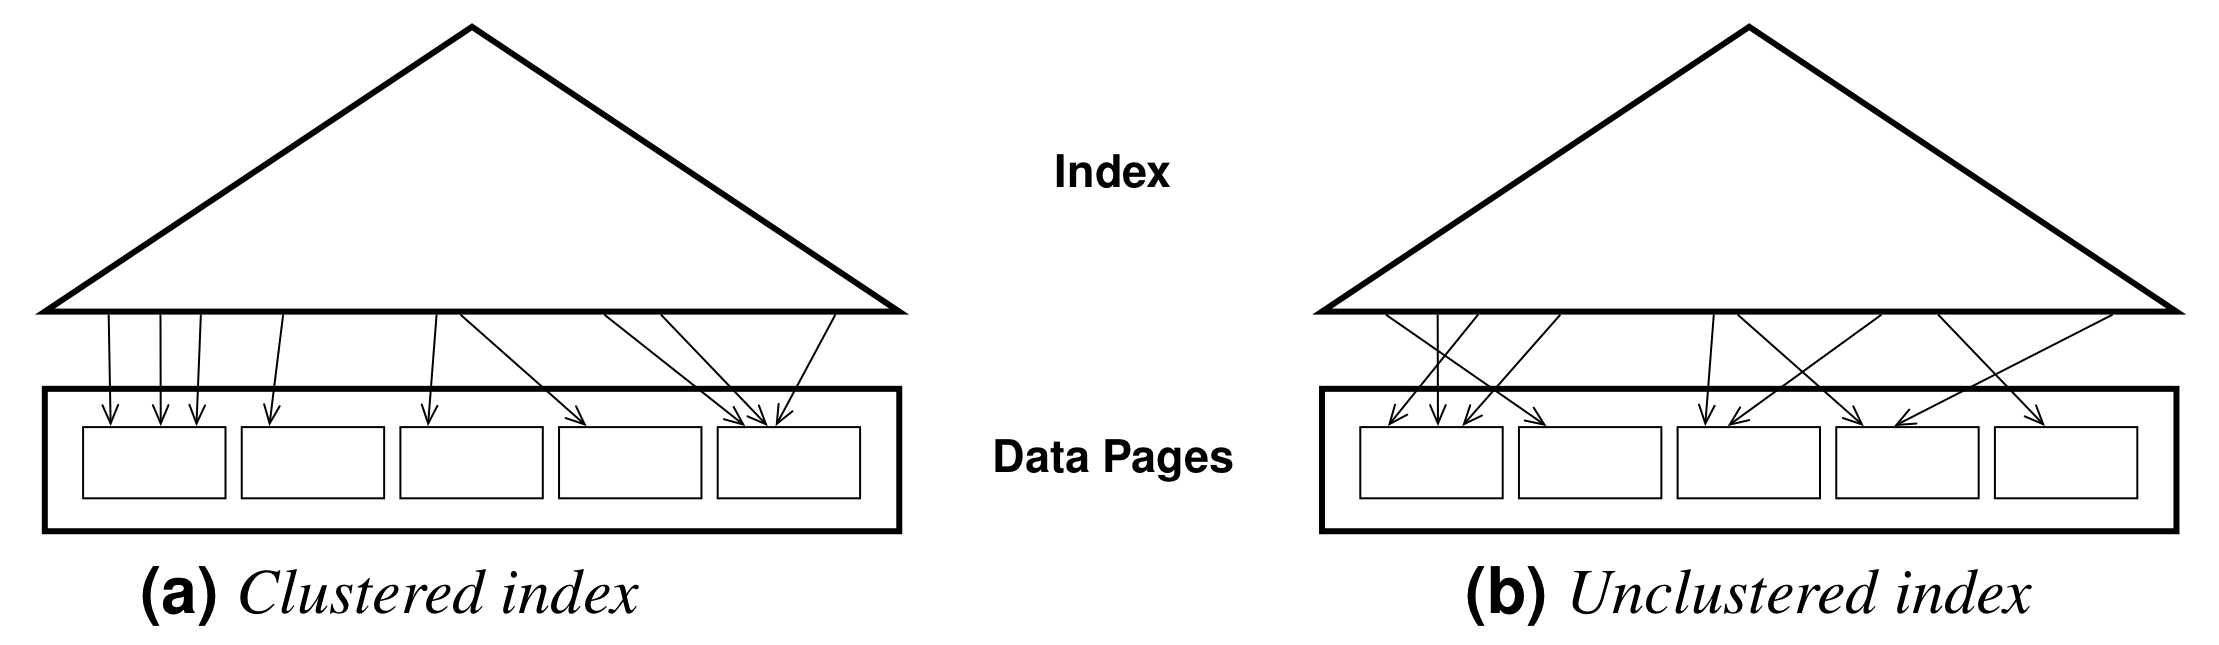
\includegraphics[width=0.7\linewidth]{images/DBMS_Internals/DynamicTreeStructureOrganizations/indexes_types.jpeg}
    \caption{Types of indexes}
\end{figure}

To support fast retrieval of records in a table using different keys, two types of indexes can be used:
\begin{itemize}
    \item If the table is stored with a \textit{heap organization}, an index is defined for each key, and the elements of the indexes are pairs \((k_i,rid_i)\) where \(k_i\) is a \textit{key value} for a record and \(rid_i\) is the record identifier
    \begin{tcolorbox}
    A \textbf{clustered index} on a key \(K\) of a table is created by first sorting the table on the values of the index key \(K\). If new records are inserted into the table after the clustered index is created, the efficiency of the index decreases. To overcome this problem we specify that a small fraction of each data page is left empty for future insertions.
    \end{tcolorbox}
    A clustered index is particularly useful for a range key search.
    \item If the table is stored with a \textit{dynamic primary organization} using the “primary key”, indexes are defined for the other keys, and the element of the indexes are pairs \((k_i, pk_i)\) where \(k_i\) is the value for a record and \(pk_i\) is the primary key value of the corresponding value
\end{itemize}

There are two additional types of indexes:
\begin{enumerate}
    \item An index on a key is called \textbf{dense} if the number of its entries is equal to the number of records stored into a separated data file
    \begin{figure}[!h]
    \centering
    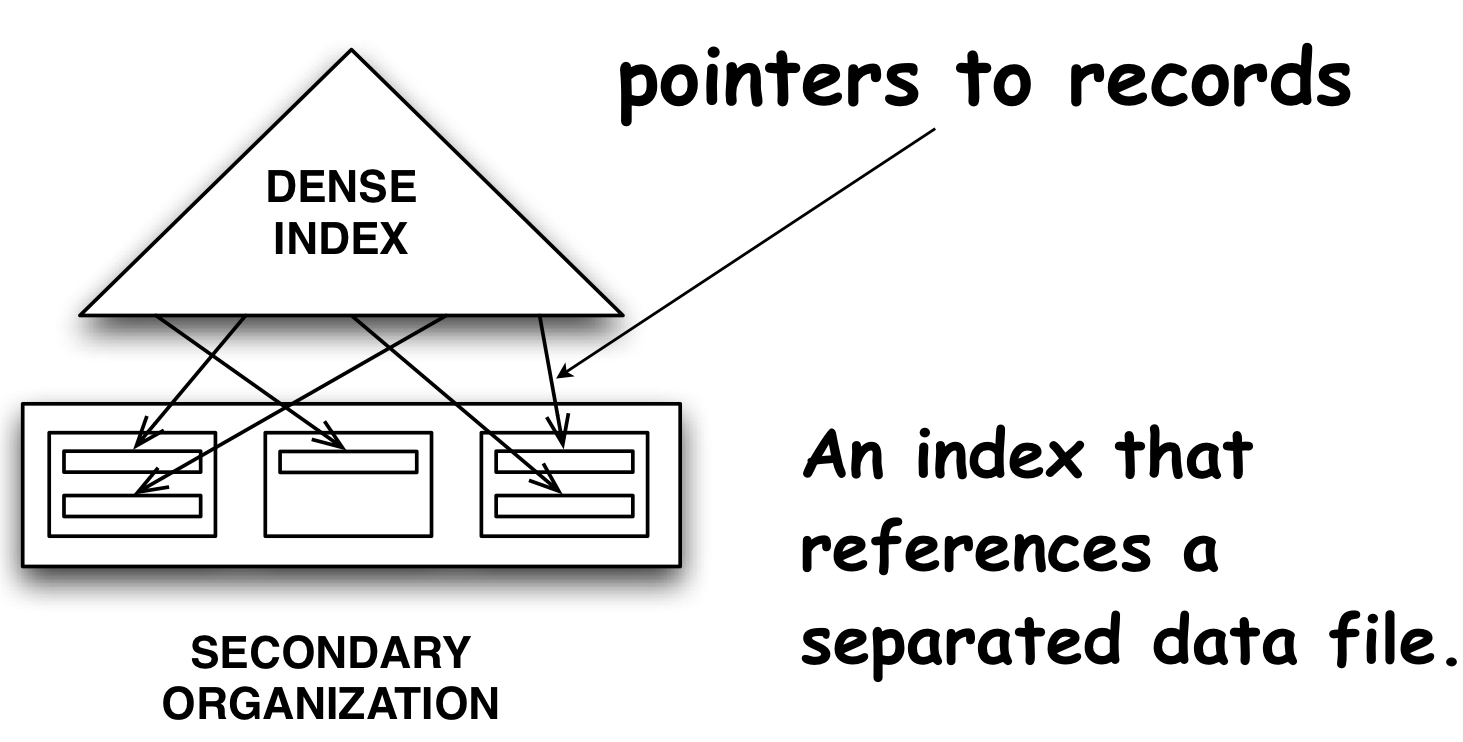
\includegraphics[width=0.5\linewidth]{images/DBMS_Internals/DynamicTreeStructureOrganizations/dense_index.jpeg}
    \caption{Dense index}
\end{figure}
    \item The term \textbf{sparse index} is used for the part of the tree structure used to locate the data records stored sorted in the leaves of a B+-tree. It is called sparse because the number of its entries is less than the number of data records
    \begin{figure}[!h]
    \centering
    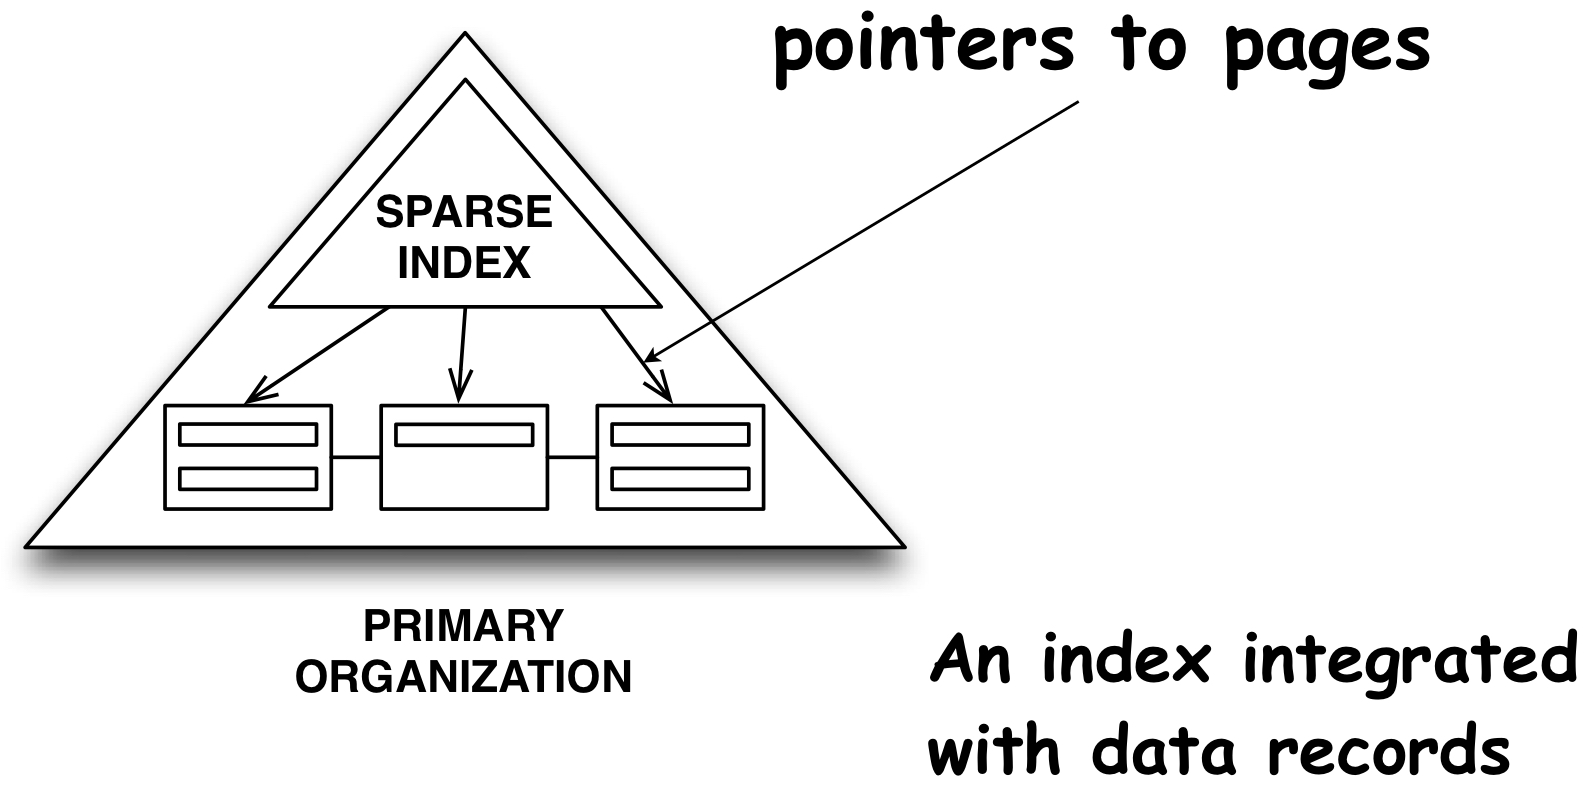
\includegraphics[width=0.5\linewidth]{images/DBMS_Internals/DynamicTreeStructureOrganizations/sparse_index.jpeg}
    \caption{Sparse index}
\end{figure}
\end{enumerate}


\subsection{Performance Evaluation - (NOT REQUIRED)}

\subsubsection{Unclustered Index}
\begin{itemize}
    \item \textbf{Search Cost:} \(C = C_i \times C_d\) = cost for index access plus cost for data access. Equal to 1 since the upper part of the index can fit in primary memory
    \item \textbf{Equality Search Cost:} \(C = 1 + 1\)
    \item \textbf{Range Search Cost:} in order to explain this we have to introduce additional measures:
    \begin{itemize}
        \item \textit{Selectivity factor:} \(sf(p)\) with \(p = v_1 < k < v_2\) is an estimate of the fraction of records which will satisfy the condition:
        \[sf(p) = \frac{v_2 - v_1}{k_{max} - k_{min}}\]
        \item \textbf{Visited leafs:} so how many pairs we can fit on the pages
        \[N_{leaf}(idx) = \Bigg\lceil \frac{L_k + L_{RID} \times N_{REC}(R)}{D_{pag} \times f_r} \Bigg\rceil\]
        \item Let us assume that the cost of an index access is estimated with the number of leaves to visit \(\lceil sf(p) \times N_{leaf}(idx) \rceil\) and the number of RID of the records that satisfy the condition is
        \[E_{rec} = \lceil sf(p) \times N_{rec}(R)\]
        \item Since the records are not sorted on the index key values, the number of pages to read is \(E_{rec}\), and therefore the search cost using the index is:
        \[\lceil sf(p) \times (N_{leaf}(idx) + N_{rec}(R))\]
    \end{itemize}
\end{itemize}

\subsubsection{Clustered Index}
\begin{itemize}
    \item \textbf{Search Cost:} \(C = Ci  Cd\) 
    \item \textbf{Equality Search Cost:} \(C = 1 + 1\)
    \item \textbf{Range Search Cost:} The records are always retrieved using the index since, although it has been constructed from sorted records, in the case of subsequent insertions it is not certain that the records are still sorted. The number of data pages to visit to find \(E_{rec}\) records is:
    \[\lceil sf(p) \times N_{pag}(R) \rceil\]
    And the overall cost of the search with the use of the index becomes:
    \[\lceil sf(p) \times (N_{leaf}(idx) + N_{pag}(R)) \rceil\]
\end{itemize}